\documentclass[11pt]{article}

\usepackage{graphicx}
\usepackage{fancyref}
\usepackage{fancyhdr}

\title{Physics 426 - Instability Notes}
\author{Jody Klymak}

\begin{document}

\maketitle
\pagestyle{fancy}
\section{Introduction}

\begin{figure}[hbtp]
  \begin{center}
    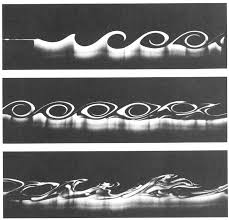
\includegraphics[width=4in]{images/Instability.jpg}
    \caption{Shear instability in a fluid; the flow in the upper half is moving to the right faster than the fluid in the lower half.   The three panels are distance downstream.}
    \label{fig:Instability}
  \end{center}
\end{figure}

We have seen in the lab demos that fluid flow is very susceptible to becoming unstable and breaking down into turbulence.  An example is shown in \fref{fig:Instability} where the flow in the upper layer is moving faster than flow in the lower layer and this leads to a "shear instability".  A few things to note:

\begin{itemize}
  \item There is clearly a preferred horizontal scale to this instability.  The billows that grow are one size until they self-interact and become turbulent.
  \item This horizontal scale must be present in the upstream conditions, but it need not be large.  
  \item The instability takes time to grow. 
\end{itemize}

This leads to a few questions we commonly ask ourselves about a flow
\begin{enumerate}
  \item Is a flow unstable? 
  \item If a flow is unstable can we say what scale has the fastest growth rate?
  \item How fast is that growth rate?   
\end{enumerate}

\section{Rayleigh Shear Instability}

As a simple situation that often leads to instability lets consider a homogeneous steady background flow $u = U(y)$.  The idea of an instability is that there are always small imperfections to this flow.  Physically, its easiest to think of these as small displacements of the streamlines around the mean and then consider what happens if there are small perturbations to the flow.  If the flow is stable, then all perturbations will be damped, whereas if it is unstable some perturbations will grow. 


\begin{figure}[hbtp]
  \begin{center}
    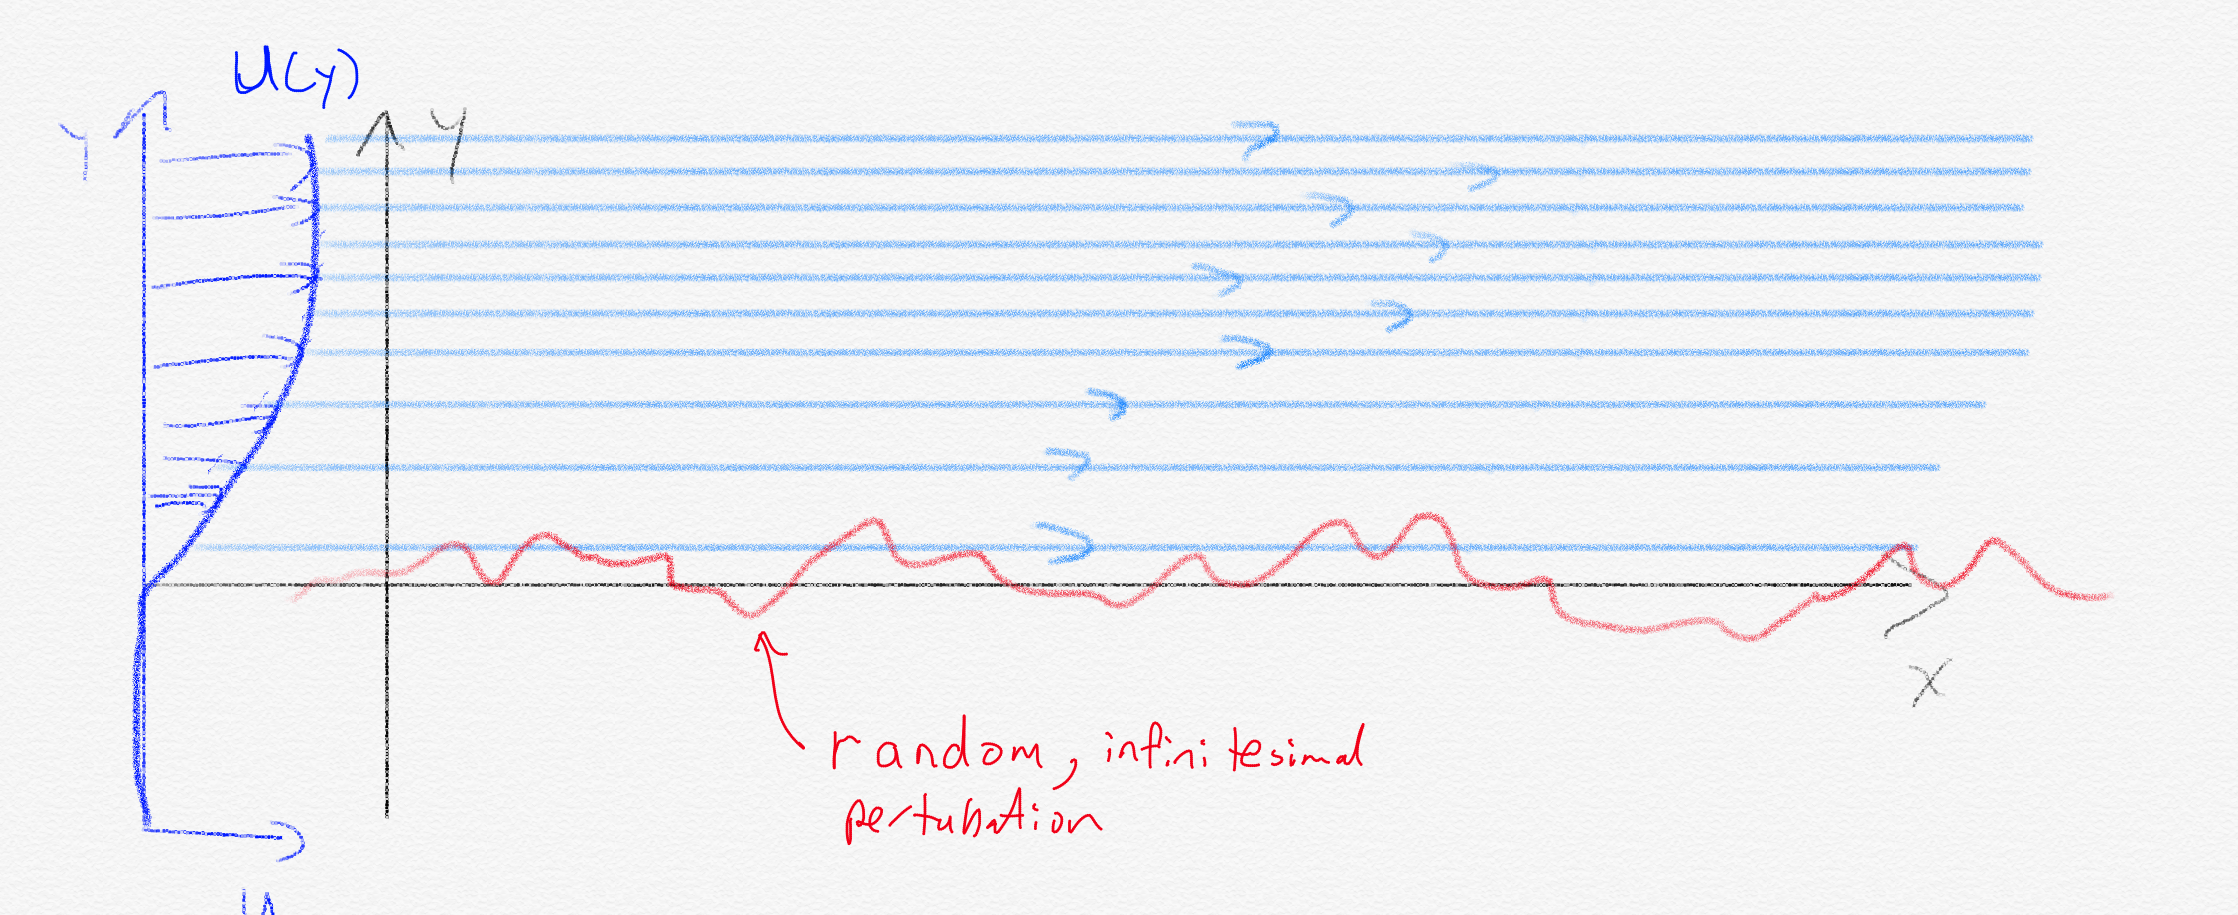
\includegraphics[width=5in]{images/ShearInstabilitySketch.png} 
    \caption{Schematic of shear instability.  Background flow is steady and has a dependence in $y$. The idea of a flow instability is to perturb the flow and see what scales in the flow grow.   }
    \label{fig:Instability}
  \end{center}
\end{figure}

\subsection{Linear perturbation analysis}

All of these methods decompose the flow into a background component of the flow and a 'perturbation', and then assume that the perturbation is small so that only linear terms in the perturbation are retained.  i.e. if $u = U(y) + u'(x, y, y)$ then terms that are quadratic or higher in $u'$ are assumed small.   So, similarly $v=v'$, and $p=p'$ because neither of these two variables have a background component. 

So for the flow above the x-, and y-momentum equations, and continuity equations become:

\begin{eqnarray*}
  \frac{\partial u'}{\partial t} + U\frac{\partial u'}{\partial x} + v'\frac{\partial U}{\partial y} & = & - \frac{1}{\rho}\frac{\partial p'}{\partial x} \\
  \frac{\partial v'}{\partial t} + U\frac{\partial v'}{\partial x} & = & - \frac{1}{\rho}\frac{\partial p'}{\partial x}\\
  \frac{\partial u'}{\partial x} + \frac{\partial v'}{\partial y} & = & 0
\end{eqnarray*}

To see how this flow behaves in the presence of perturbations, we assume the flow is a periodic travelling wave in the x-direction and has a y-direction structure (to be determined):

\begin{eqnarray*}
  u' &= &\hat{u}(y)\ e^{i k (x -ct)}\\
  v' &= &\hat{v}(y)\ e^{i k (x -ct)}\\
  p' &= &\hat{p}(y)\ e^{i k (x -ct)}\\
\end{eqnarray*}

This gives three coupled PDEs for the vertical structure of the response that depends on $k$ and $c$:

\begin{eqnarray*}
-ikc\ \hat{u} + ik U\ \hat{u} + U'\ \hat{v} & = & -ik\ \hat{p}\\
-ikc\ \hat{v} + ik U\ \hat{v}  & = & -ik\ \frac{\partial \hat{p}}{\partial y}\\
ik\ \hat{u} + \frac{\partial \hat{v}}{\partial y} & = & 0
\end{eqnarray*}
where here we have defined $U' \equiv \frac{\partial U}{\partial y}$.

This is three coupled equations in three unknowns, so as usual we combine, choosing to do so for $\hat{v}(y)$, and after some algebra get

\begin{equation}
\label{eq:Rayleigh}
  \hat{v}'' + \hat{v}\left(\frac{U''}{c-U} - k^2\right) = 0
\end{equation}

How does this help us?  \Fref{eq:Rayleigh} cannot be solved analytically, but as we will see below some useful criteria for stability can be derived analytically using it.  However, first what is the character of the numerical solutions?  We note that $k$ is always real (its the wavelength of the disturbance we are interested in), but that $c$ may be imaginary in general.  If it is imaginary, then we have growing solutions if $\mathcal{I}(c) < 0$ (assuming $k>0$) and the growth rate will be given by $k\mathcal{I}(c)$.

Now all we need to do is solve for $c$ and $\hat{v}(y)$ for a given $U(y)$ and $k$. \Fref{eq:Rayleigh} is a classic eigenvalue problem, where $c$ can have a number of distinct values for a given background profile of $U(y)$.  When we solve this numerically, the numerical solution ends up being a matrix eigenvalue problem.  

\subsection{Numerical Solution}

Numerically \fref{eq:Rayleigh} is straightforward to set up using first differencing.  First we rewrite in an eigen-vector/eigen value form, where $\hat{v}(y)$ are the eigen vectors and $c$ are the eigenvalues:
\begin{equation}
  \left[ \left(\frac{\partial^2}{\partial y^2} - k^2\right) U - U''\right]\hat{v} = c \left[ \frac{\partial^2}{\partial y^2} - k^2\right] \hat{v} 
\end{equation}
We write it this way because that allows us to write the discretized form as matrix equation of the form 

\begin{equation}
 A \mathbf{v} = c B \mathbf{v}
\end{equation}
where $A$ and $B$ are matrices, and $\mathbf{v}$ is an eigenvector we are solving for and $c$ is a \emph{generalized} eigenvalue problem for which there are numerical solvers in most linear algebra packages (i.e. \texttt{scipy.linalg.eigh}).  

Setting up the matrices $A$ and $B$ is straight forward based on our previous discretization attempts.  If divide the y-domain into $N$ grid points, indexed from $0$ to $N-1$, then we end up with two tri-diagonal matrices: 
\begin{eqnarray*}
  A_{i, i-1} = A_{i, i+1} & = & U_i / \Delta y^2\\
  A_{i, i} & = &  \left(-2 /\Delta y^2 -k^2\right)U_i -(U_{i+1} + U_{i-1} -2 U_i)/\Delta y ^2\\
\end{eqnarray*} 
and for $B$:
\begin{eqnarray*}
  B_{i, i-1} = B_{i, i+1} & = & 1 / \Delta y^2\\
  B_{i, i} & = &  -2 /\Delta y^2 -k^2 \\
\end{eqnarray*} 
These relationships are for interior points where $i>0$ and $i<N-1$.  For the first and last row we need to assume boundary conditions, which in this case is the disturbance goes to zero at the boundaries: $\hat{v}_{-1} = \hat{v}_{N} = 0$, and assume that $U$ has not gradient there: $U_{-1} = U_0$ and $U_{N} = U_{N-1}$.  If we do that then we just plug those values into the above relations to get 
\begin{eqnarray*}
A_{0, 0} &=& \left(-2 /\Delta y^2 -k^2\right)U_0 -(U_1 - U_0)/\Delta y ^2\\
A_{0, 1} & = &U_0/\Delta y^2\\
B_{0, 0} & = &  -2 /\Delta y^2 -k^2 \\
B_{0, 1} & = & 1 / \Delta y^2
\end{eqnarray*}
and similarly for $i=N-1$.   

This eigenvalue problem can then be solved for each value of $k$ to be explored, and the fastest growing unstable mode determined for each $k$.  An example of this calculation is shown for the profile in \fref{fig:VelocityProfile}.  There is a clear minimum in the growth time for this profile at $k=2.3\times10^{-4}\ \mathrm{rad\,m^{-1}}$ indicating that this wavelength will have the fastest growing instability.  The shape of the eigenvectors (\fref{fig:EigenVectors}) can also be determined if that is of interest.        

\begin{figure}[hbtp]
  \begin{center}
    \includegraphics[width=4in]{../python/VelocityProfile.pdf}
  \end{center}
    \caption{Background velocity profile for stability analysis.}
    \label{fig:VelocityProfile}
\end{figure}

\begin{figure}[hbtp]
  \begin{center}
    \includegraphics[width=4.5in]{../python/GrowthRate}
  \end{center}
  \caption{a) Fastest-growing eigenvalue and b) growth timescale as a function of wavenumber for the velocity in \fref{fig:VelocityProfile}.  The fastest growing wavenumber is broadly around 25-km scale.}
  \label{fig:GrowthRate}
\end{figure}

\begin{figure}[hbtp]
  \begin{center}
    \includegraphics[width=4in]{../python/EigenVectors.pdf}
  \end{center}
  \caption{Eigenvectors for discrete wavenumbers $k$.  The eigenvectors with solid colours are unstable, and the dashed ones are stable.}
  \label{fig:EigenVectors}
\end{figure}

\clearpage
\subsection{Fully non-linear simulation}

The same velocity profile can be used as the initial conditions of a primitive equation numerical model.  Here we set up a channel that has solid boundaries in $y$ and is periodic in $x$ over a distance of 400 km (\fref{fig:ChanPar01}) and use the same velocity profile as \fref{fig:VelocityProfile}.  The flow is seeded with very small imperfections that then grow or are suppressed.  We can see the growth starting in \fref{fig:ChanPar01}b.  

\begin{figure}[hbtp]
  \begin{center}
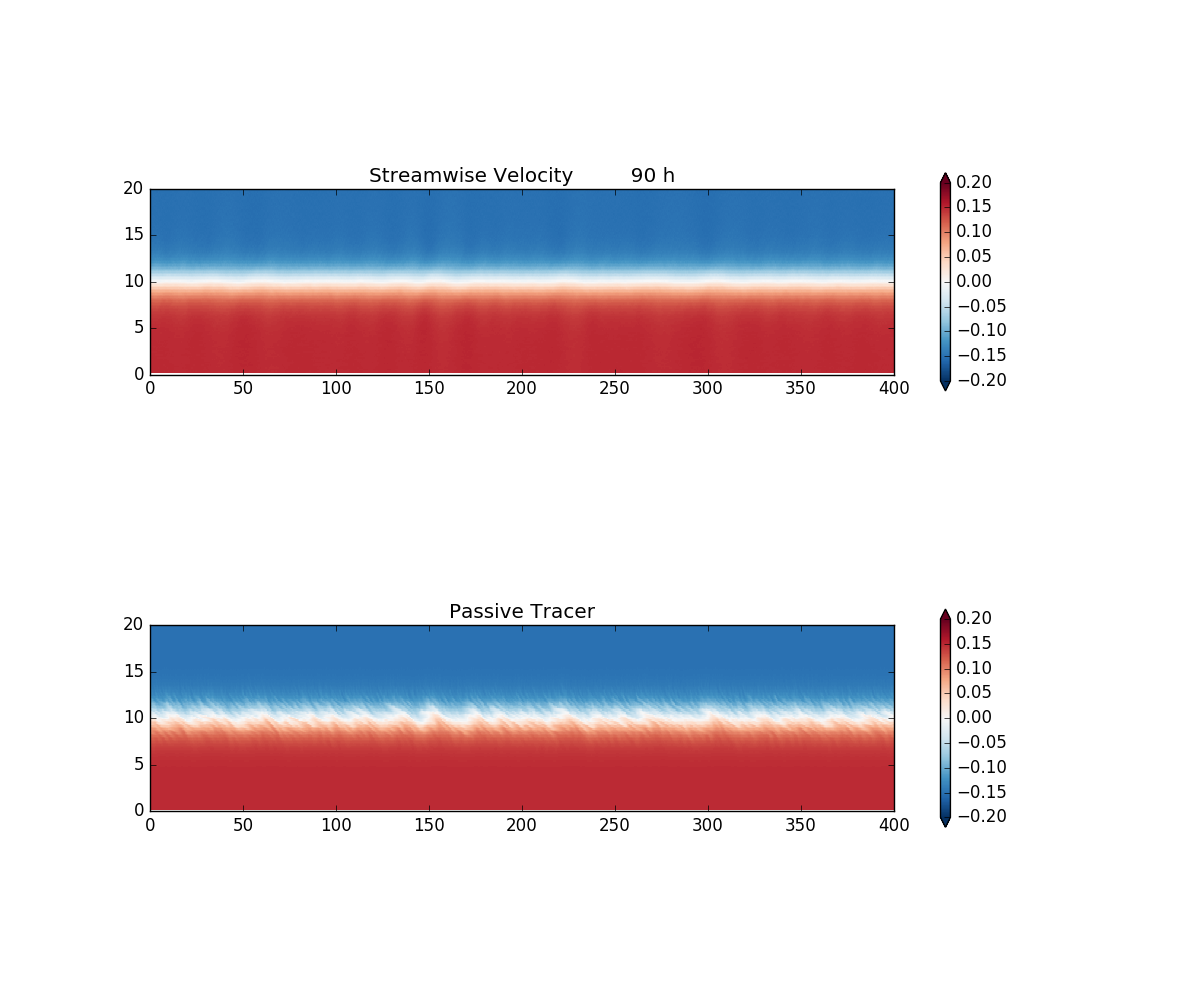
\includegraphics[width=5in]{images/ChanPar040000324000}
  \end{center}
  \caption{Channel simulation with shear as in \fref{fig:VelocityProfile}, and some added numerical noise after it has been allowed to evolve for 90 h.  Upper plot is velocity, and lower plot is a passive tracer with the same initial distribution as the velocity }
  \label{fig:ChanPar01}
\end{figure}

After the flow has evolved for longer (160h) than the fastest growth scale, it is clear that a scale of about 25 km has been "selected" in the flow instability (\fref{fig:ChanPar02}).  The other scales are still present, but did not grow as fast as this scale and hence it dominates the figure.  Its worth noting that the billows in this simulation are all slightly different, and that is the chaotic amplification of slightly different-phased disturbances.  

\begin{figure}[hbtp]
  \begin{center}
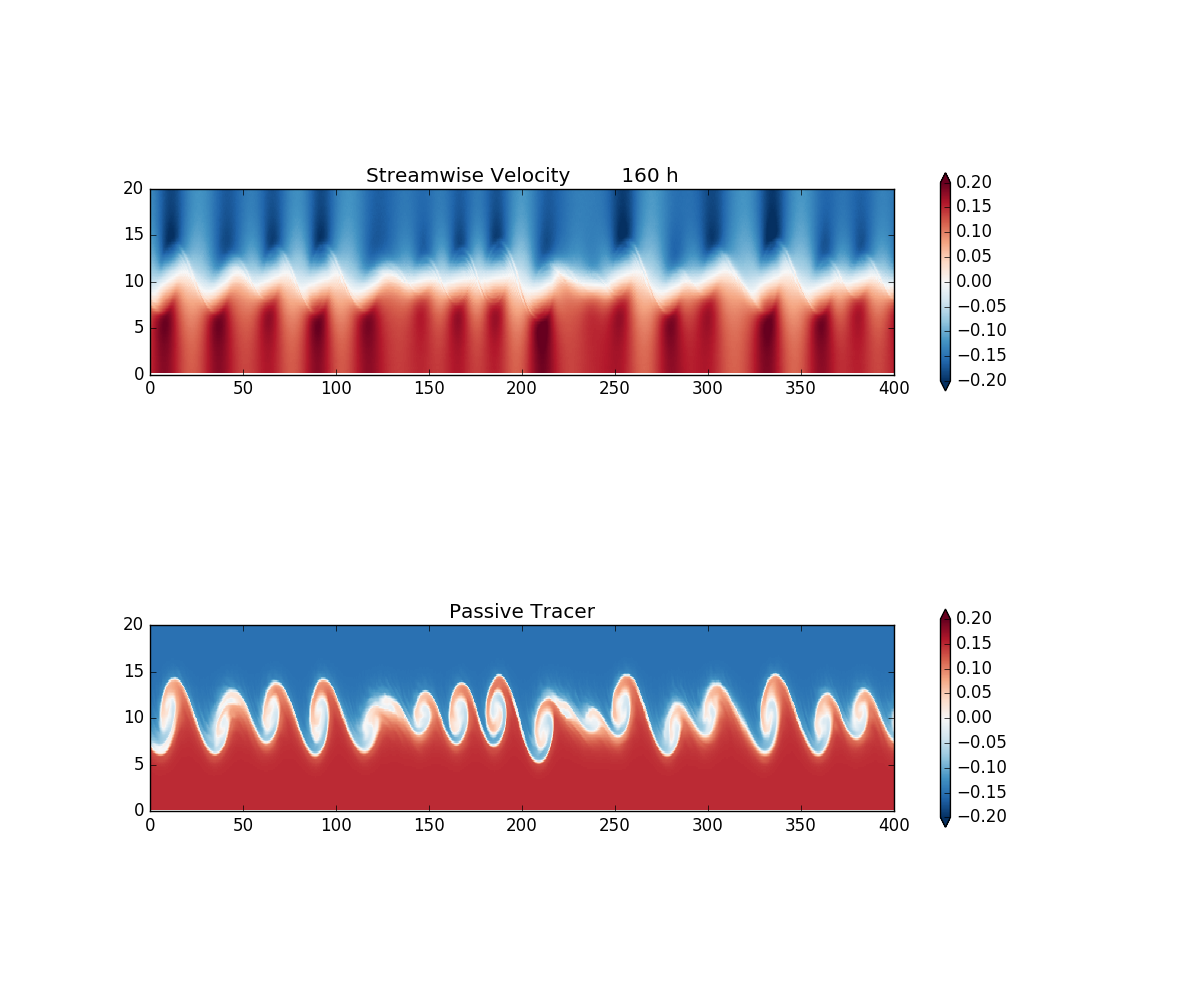
\includegraphics[width=5in]{images/ChanPar040000576000}
  \end{center}
  \caption{As \fref{fig:ChanPar01} except after 160 h, when the instabilites have grown to noticeable size.}
  \label{fig:ChanPar02}
\end{figure}

\clearpage

As the flow evolves for a longer period of time, these un-even vortices start to self-interact, and pairs of vortices merge to create larger channel-spanning vortices (\fref{fig:ChanPar03}).  These eventually completely collapse into near-homogeneous turbulence.

\begin{figure}[hbtp]
  \begin{center}
    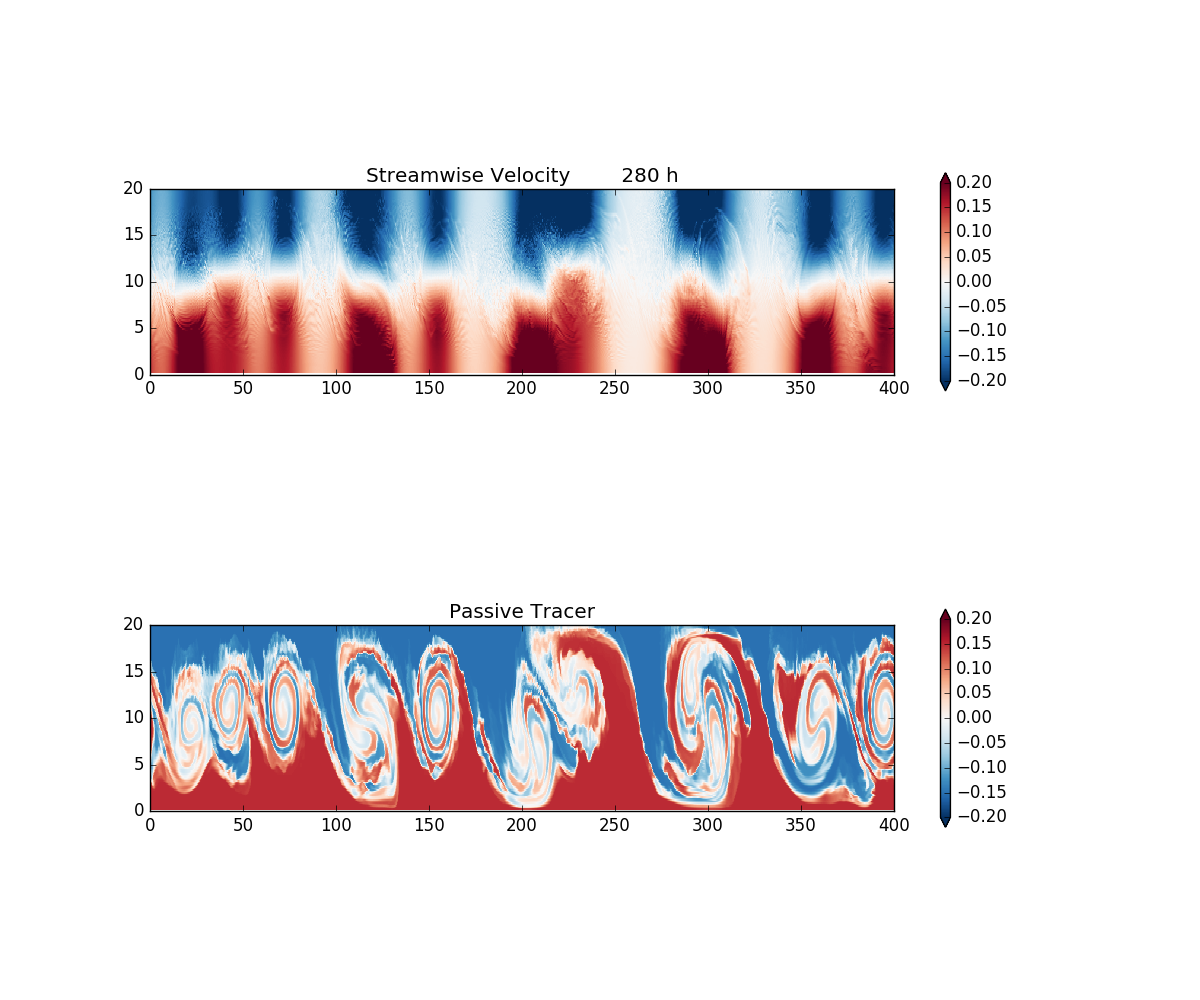
\includegraphics[width=5in]{images/ChanPar040001008000}
  \end{center}
  \caption{As \fref{fig:ChanPar01} except after 160 h, when the instabilites have grown to noticeable size.}
  \label{fig:ChanPar03}
\end{figure}
   
\clearpage

The evolving character of the flow is well-visualized by looking at spectra of the tracer variance in the along-stream direction (\fref{fig:ShearSpectra}).  Note that the fastest-growing wavenumbers are near the wavenumber predicted by the linear perturbation theory ($k = 0.036\ \mathrm{cpkm} = 2.3\times10^{-4}\ \mathrm{rad/m}$).

\begin{figure}[hbtp]
  \begin{center}
    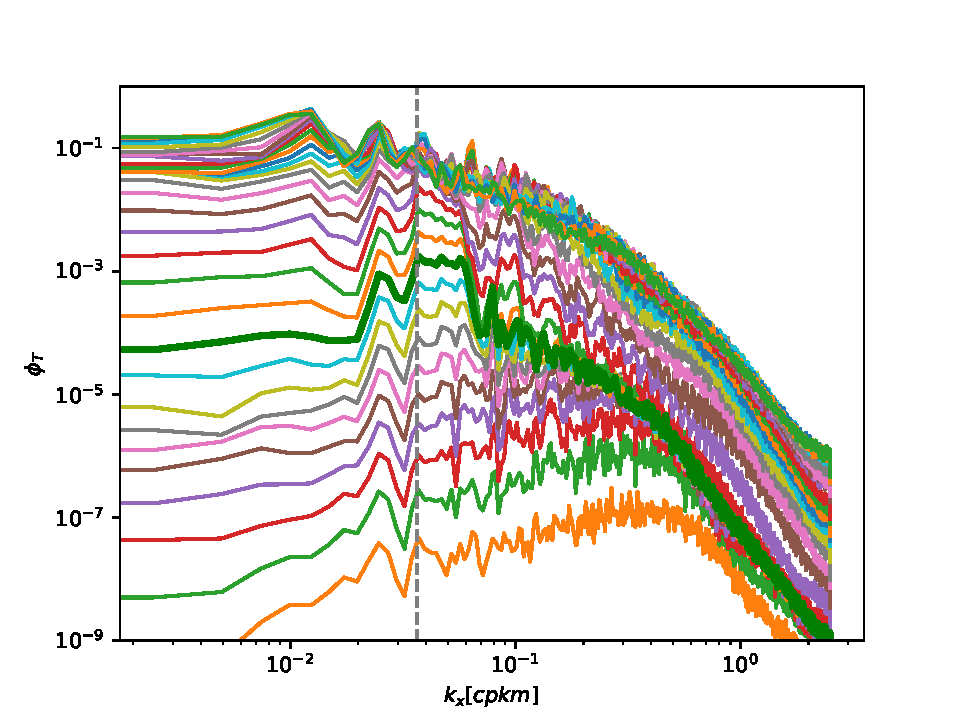
\includegraphics[width=5in]{images/ShearSpectra.pdf}
  \end{center}
  \caption{Spectra of tracer variance in the along-flow direction. Spectra with more variance are from later in the simulation.  Note the broad peak near the wavenumber of the fastest-growing mode (grey dashed line)}
  \label{fig:ShearSpectra}
\end{figure}

Note that there is a steep roll-off of the tracer spectrum to high wavenumbers.  This is a rough approximation of the inertial and convective subranges of turbulence, where I say they are rough because the numerics are such that the Reynolds number of these flows is not very high. 

\clearpage

\subsection{Stability of flows}

We chose the flow in the examples above to be unstable.  Consider a different example (\fref{fig:RayleighInstabilityStable}) and note that the growth rate for the unstable mode is many thousands of hours.  A primitive equation simulation of this flow never develops instability because any disturbances that form are killed by viscosity in the model before they have a chance to grow.  Indeed the fact that we found a finite timescale for the growth of this mode is just a numerical artifact, and can be made arbitrarily long if we increase the vertical resolution of the numerical discretization.  

\begin{figure}[hbtp]
  \begin{center}
    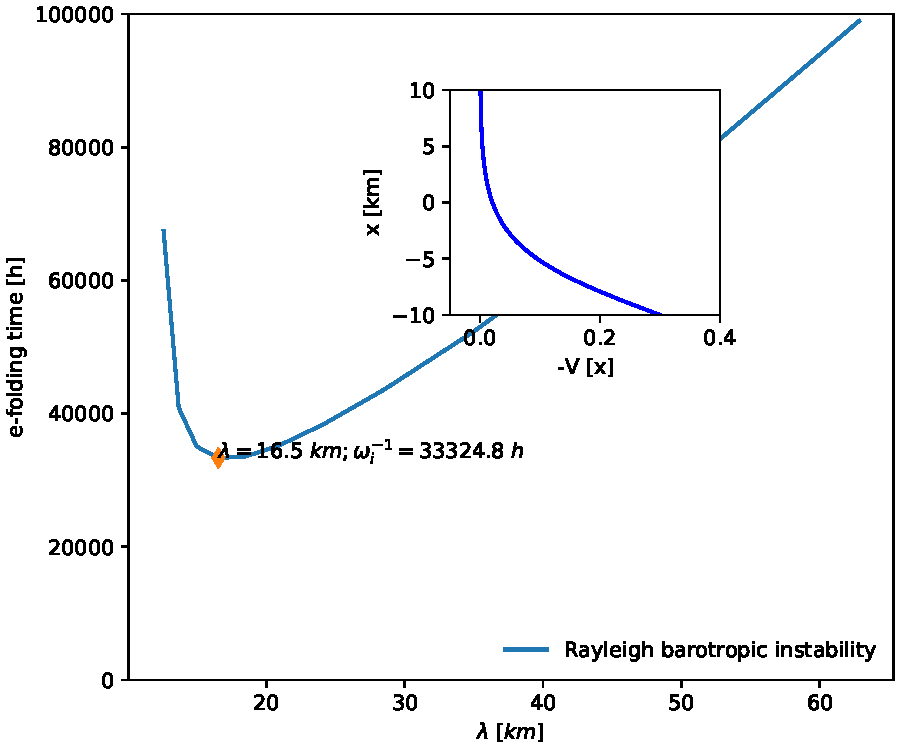
\includegraphics[width=4in]{images/RayleighInstabilityStable.pdf}
  \end{center}
  \caption{Unstable mode growth rate for profile in the inset.  Note that it is many thousands of hours, and hence effectively infinite.}
  \label{fig:RayleighInstabilityStable}
\end{figure}

It turns out that we can mathematically see which background flows $U(y)$ are stable or unstable, which is of course very useful, and often one of the primary goals of stability analysis.  Reconsider \fref{eq:Rayleigh} by multiplying by the complex conjugate of $\hat{v}$, $v^*$ and integrate across the y-domain:

\begin{equation}
    \int_{0}^L v^{*}\hat{v}'' \ \mathrm{d}y +  \int_{0}^L v^{*}\hat{v}\left(\frac{U''}{c-U} - k^2 \right) \ \mathrm{d}y  = 0
\end{equation} 
Note that integrating by parts yields: $\int_{0}^L v^{*}\hat{v}''  = v^{*}v'|^{L}_0 - \int_{0}^L |v'|^2\ \mathrm{d}z$ so that we can rewrite as 
\begin{equation}
    \int \left(|v_y|^2  + k^2|v|^2 \right)\ \mathrm{d}y + \int \frac{U''}{U-c} |v|^2 \ \mathrm{d}y = 0
\end{equation}
The first term is always real.  The second term is only imaginary due to the presence of $c$ in the denominator, so multiplying top and bottom by the complex conjugate $U-c^*$, the imaginary part is
\begin{equation}
    c_{I}\int \frac{U'' |v|^2}{|U-c|^2}\ \mathrm{d}z = 0
\end{equation}
So, if $c_I$ is not zero then the integral must be zero, but the only thing that can change sign is $U''$ so we can reach the conclusion that the flow is stable is $U''$ does not change sign, i.e. if the curvature of $U(y)$ doesn't change somewhere in the domain.  


Hence in the examples above, The first velocity profile (\fref{fig:VelocityProfile}) \emph{can} be unstable because $U$ has negative curvature above $y=0$ and positive below $y=0$.  Note that just because it \emph{can} be unstable doesn't mean it will be, but the instability analysis proves that it is.  Conversely, the velocity profile used in \fref{fig:RayleighInstabilityStable} only has negative curvature, i.e. the sign of $U''$ does not change in the channel.  Therefore that flow cannot be unstable, and the numerical stability analysis and simulations reflect this.  


\section{Stratified Shear (Kelvin-Helmholtz) Instability}

\begin{figure}
\begin{center}
  \includegraphics[width=4.5in]{images/KHBillows}  
\end{center}
\caption{Kelvin-Helmholtz billows observed in the atmosphere, and visualized with clouds}
\end{figure}

A second type of shear instability is the shear between two immiscible layers $\rho_1$ and $\rho_2$ with a background flow that is at a different speed.  The text follows a version where the layers are of infinite thickness, which is a bit more analytically tractable than allowing variable depth like we did in class.  For this case, we assume the flow on either side of the interface is irrotational and divide into a base state and a fluctuating component.  Because the flow is irrotational, the velocity potential in each layer follows Laplace's equation.  The method of solution follows in the text ("Kelvin-Helmholtz Instability") and we won't repeat the math here.  However, the same procedure is used as before, and the velocity potentials $phi_1$ and $phi_2$ each have a vertical dependence that given the boundary conditions take the form of decaying exponentials, and sinusoids in x and t.  One gets a dispersion relation relating $c$ and $k$ for any disturbance:

\begin{equation}
  c  = \frac{\rho_2 U_2 + \rho_1 U_1}{\rho_2 + \rho_1} \pm \left[\frac{g}{k}\frac{\rho_2 - \rho_1}{\rho_2+\rho_1} - \rho_1\rho_2\left(\frac{U_1 - U_2}{\rho_1 + \rho_2} \right)^2 \right]^{1/2}
\end{equation}

which has imaginary roots, and thus is unstable if 
\begin{equation}
  g\left(\rho_2^2 - \rho_1^2 \right) < k\rho_1\rho_2\left(U_1-U_2\right)^2
\end{equation}

Note that for any given flow there is always a $k$ large enough that this is true, but in practical cases, if the scale is small enough (high enough $k$) then viscosity acts to suppress the growth of the instability.  Note the exception is if $U_1=U_2$, in which case the flow is always stable if $\rho_2 > \rho_1$.  

Also note that the stronger the density difference, the smaller scale the growing mode.  Conversely, the stronger the shear $U_1-U_2$, the easier it is.  So we often think of stratified shear instability as a competition between shear producing the turbulence, and the stratification difference between the layers suppressing it.  

Finally note that if $\rho_1 = \rho_2$, then flow is always unstable if the two layers have different flow speeds ($c = (1/2)\left((U_1 + U_2)\pm i(U_1-U_2)\right)$); such flows are called a "vortex sheet".  

As shown in the text, or videos posted on the course website, these instabilitites are relatively easy to make both in nature and the lab.  Density differences in the fluid naturally give rise to shear in the layers, whereas in the homogenous shear instability discussed previously, the shear would have to be imposed somehow, often via a splitter plate in the flow.  Nature doesn't have many splitter plates, so stratified shear instability is a more natural way to create instability.  

\section{Instability in viscous boundary layers}

We saw in the section on boundary layers that viscosity produces the Blasius profile.  If such a profile were not subject to viscous effects, then the profile that is formed would be stable.  However, viscosity is clearly non-negligible in such flows.  Similarly, we usually think of viscosity as suppressing the growth of instabilities because it damps the growth of the perturbations that arise.

However, clearly at high enough Reynolds numbers this intuition breaks down and boundary layers develop turbulence.  For pipe flow its found that for $Re>3000$ the flow will transition to turbulence, though if you are very careful the transition can be delayed until the Reynolds number is another order of magnitude larger.  The reason is almost certainly that the non-linear terms matter and a linear perturbation analysis drops too much physics from the problem.   The linear perturbation analysis is quite successful at inviscid problems, but has trouble making simple predictions for viscous problems. 



\end{document}

